\documentclass[12pt]{article}

\usepackage{sbc-template}
\usepackage{graphicx,url}
\usepackage[latin1]{inputenc}  

\usepackage{../Utils}
\usepackage{implementation}     
\sloppy

\title{Beyond ASCII -- Parsing Programs with Graphical Presentations}

\author{Martijn M. Schrage\inst{1}, S. Doaitse Swierstra\inst{1}}


\address{Department of Information and Computing Sciences\\
         Utrecht University\\
         Utrecht, The Netherlands
  \email{\{martijn,doaitse\}@cs.uu.nl}
}

\begin{document} 

\maketitle

\begin{abstract}

Proxima is a generic editor suitable for a wide range of structured document types. It allows edit operations on the document structure as well as on its screen representation (i.e.\ free-text editing) without the need to switch between the two modes. The system maintains a bidirectional mapping between the document structure and its presentation. Besides obvious applications, such as word-processor and spread-sheet editors, the system is especially well-suited for defining source editors for programming languages.

Presentation-oriented edit operations require that an edited presentation can be parsed to yield an updated document structure. However, conventional parsing techniques cannot readily be applied, since presentations in Proxima are not restricted to text but may also contain graphical elements. For example, an exponential may be presented as $3^2$. Although this graphical presentation may not be directly edited at the presentation level, its components may. Hence, instead of simply parsing the changed representation, we have to take into account the existing structure. 

This paper explains the scanning and parsing process for presentations that are a possibly nested combination of text and graphical elements. For textual parts of the presentation a Haskell combinator parser needs to be provided. The parser for graphical parts, on the other hand, is constructed by Proxima, based on information in the presentation. White space in the presentation can be handled automatically, if desired. 
\end{abstract}


\section{Introduction}\label{sect:introduction}

% what is Proxima
Proxima~\cite{schrage04Proxima} is a generic structure editor suitable for a wide range of structured document types. Its key feature is the modeless combination of structural editing and presentation editing. Figure~\ref{fig:heliumEditor} is a screenshot of Proxima at work, showing an editor for the functional programming language Helium~\cite{heeren03helium}. The editor shows inferred type signatures and provides a list with type information for the identifiers in scope. Note that various graphical presentations of code fragments are supported, as shown in the declaration of \p{f}.


\begin{figure}[ht]
\centering
\includegraphics[width=0.7\textwidth]{images/HeliumEditor}
\caption{An editor for Helium.}
\label{fig:heliumEditor}
\end{figure}


When editing program code, a structure-based view of the text often comes in handy. One might want to select a complete  function, or a subexpression, by a simple gesture, being assisted by an editor that knows the structure of the document. We refer to such edit operations as {\em structural} edit operations.

On the other hand, not all {\em presentation-oriented} edit operations correspond to meaningful operations on the document. If, for example, the middle part of the expression $(1+\framebox{$\,2) \times ($}\,3+4)$ is deleted, we again get a correct expression $(1+3+4)$. This edit operation does not directly correspond to a structural edit operation.


In order to support editing on both the document structure and the presentation, Proxima maintains a bidirectional mapping between two data structures: the structural description of the document, and its actual presentation on the screen. This mapping is described as a composition of a number of smaller mappings, several of which are parameterized by so called {\em sheets}. Together with a document type definition, these sheets form the instantiation of an editor. By supplying a document type, a presentation sheet, and a scanner and parser, a syntax-aware editor may be constructed with little effort.


% example of structural and presentation oriented editing
% define terms
% nesting

To illustrate the scanning and parsing process, we focus on a small example. Figure~\ref{fig:graphicalDecl} shows a declaration that has a mixed textual and graphical presentation. The fraction and the exponentiation both have a graphical presentation, which we will refer to as a {\em structural} presentation. In contrast, textual presentations are denoted by the term {\em parsing} presentations. 

The figure shows that a parsing presentation may contain structural presentations (e.g.\ the parsing presentation of the declaration contains a structural fraction), and ,vice versa, that structural presentations may contain parsing presentations. The fraction, for example, has parsing presentations for the numerator and the denominator (the latter one containing a structural presentation for the exponentiation again).


\begin{figure}
\begin{center}
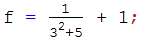
\includegraphics[width=1in]{images/scanFrac}\
\end{center}
\caption{A graphically presented declaration.} \label{fig:graphicalDecl} 
\end{figure}



% presentations are textual, or graphical (call it structural). Cannot edit this one. children can be

Because of the complexity of parsing a structural presentation and defining a meaningful subset of edit operations, Proxima disallows presentation editing on structural presentations. Any parsing subpresentation (such as the numerator and denominator in the fraction), however, is editable again. Hence, in Figure~\ref{fig:graphicalDecl} we can type \p{+1} next to the \p{1} in the numerator, but we cannot delete the horizontal line. We can delete the entire fraction though, by putting the caret after it and pressing backspace. A fraction may be introduced using a menu, or by typing a `$/$' operator, which is replaced by a graphical fraction after the next successful parse. 
%\todo{low priority: also say that / remains until parsing after which focus is restored?}

Summarizing, we have two kinds of presentations:

\bl
\o {\bf Parsing presentation} A presentation that contains consists of text and possible structural presentations. It supports structure editing as well as presentation editing.
\o {\bf Structural presentation} A possibly graphical presentation that does not support presentation editing. It may have either structural or parsing child presentations, with the latter supporting presentation editing again.
\el


After the presentation of a document has been edited, the modified presentation needs to mapped back onto a structured document. However, due to the mix of structural and parsing presentations, conventional parsing methods cannot readily be used. In this paper, we show how the scanner and parser layers of Proxima co-operate in this reverse mapping. 

Figure~\ref{fig:scanResult} shows the result of the Proxima scanner when it is applied to the presentation in Figure~\ref{fig:graphicalDecl}. It consists of a nested structure of \p{ParsingTk} tokens and \p{StructuralTk} tokens that matches the structure of the presentation. Textual tokens are represented by \p{UserTk} tokens. Each token has a unique number, which is denoted by a subscript, and is referred to as its {\em presentation identity}. Presentation identities have type \p{IDP} and are used to associate a token with its white space. In addition to a sequence of tokens that represent its children, a structural token also contains the structured document fragment it represents. This document fragment is necessary because sometimes a structural presentation does not contain enough information to reconstruct the document tree. (A \p{ParsingTk} token also contains such a document fragment, and an additional parser, but for brevity, these are not shown in the figure.) Together with the tokens, the scanner produces a {\em white-space map}: a mapping between a token's presentation identity and its trailing white space.


\begin{figure}
\begin{footnotesize}
\begin{tabbedCode}
ParsingTk$_0$ \= \\
~~ \= [ UserTk$_1$ (IdentToken "x") \\
   \> , UserTk$_2$ (OpToken "=") \\
   \> , StructuralTk$_3$ (DivExp (IntExp 1) (PlusExp ...))\\
   \> ~~~~ \= [ ParsingTk$_4$ [ UserTk$_5$ (IntToken 1)] \\
   \>      \> , ParsingTk$_6$ \= [ StructuralTk$_7$ (PowerExp (IntExp 3) (IntExp 2))\\
   \>      \>              \> ~~~~ \= [ ParsingTk$_8$    \= [ UserTk$_9$ \= (IntToken 3) ] \\
   \>      \>              \>      \> , ParsingTk$_{10}$ \> [ UserTk$_{11}$  \> (IntToken 2) ] ]\\
   \>      \>              \> , UserTk$_{12}$ (OpToken "+") \\
   \>      \>              \> , UserTk$_{13}$ (IntToken 5) ] ] \\
   \> , UserTk$_{14}$ (OpToken "+") \\
   \> , UserTk$_{15}$ (IntToken 1) \\
   \> , UserTk$_{16}$ (SymToken ";") ]\\
\\
whitespaceMap ::~IntMap IDP (NrOfBreaks, NrOfSpaces)\\
whitespaceMap = [$1 \mapsto (0,1),~2 \mapsto (0,1),~3 \mapsto (0,1),~14 \mapsto (0,1),~16 \mapsto (1,0)$]
\end{tabbedCode}
\end{footnotesize}
\caption{A scanned declaration.} \label{fig:scanResult} 
\end{figure}

%\todo{explain that all tokens in a parsingTk contain refs to their originating nonterminal in the document?}
% In case of incomplete presentation, we reuse the fields from that node. Fragile. Copy/paste, retyping, it may get lost. So only for non-essential things. 

Parsing the token structure in Figure~\ref{fig:scanResult} is relatively straightforward. For the parsing parts, we use a combinator parser that has a special primitive for structural tokens. The presentation sheet specifies which parser is to be used. The structural parts, on the other hand contain enough information to be parsed without the need to specify a parser.

The paper is organized as follows. We start by providing a brief overview of Proxima's architecture (Section~\ref{sect:architecture}) and the kind of document types that can be defined (Section~\ref{sect:documentStructure}). Then we explain the components and data types involved in computing the presentation of a document in Section~\ref{sect:presentationProcess}. The Proxima scanning and parsing algorithms are explained in sections~\ref{sect:scanner} and~\ref{sect:parser}, and form the core technical content of this paper. Section~\ref{sect:relatedWork} describes related work, and Section~\ref{sect:conclusion} concludes.






%%%%%%%%%%%%%%%%%%%%%%%%%%%%%%%%%%%%%%%%%%%%%%%%%%%%
%
\section{The architecture of Proxima} \label{sect:architecture}
%
%%%%%%%%%%%%%%%%%%%%%%%%%%%%%%%%%%%%%%%%%%%%%%%%%%%%

The core architecture of Proxima consists of a number of layers, each communicating with its direct neighbors. The layered structure is based on the staged nature of the {\em presentation} process and its inverse, the {\em interpretation} process. The positions at which the document, the rendering, and the intermediate data structures reside are called {\em levels}. Between each pair of levels we have a {\em layer} that maintains the mappings between its adjacent levels. Each layer consists of a presentation component and an interpretation component and may be parameterized by a {\em sheet}. Figure~\ref{fig:levelsAndLayers} schematically shows the levels and layers of Proxima. From a document type definition and the sheets, a number of Haskell modules are generated, which are compiled to yield an editor.


\begin{figure}[ht]
\centering
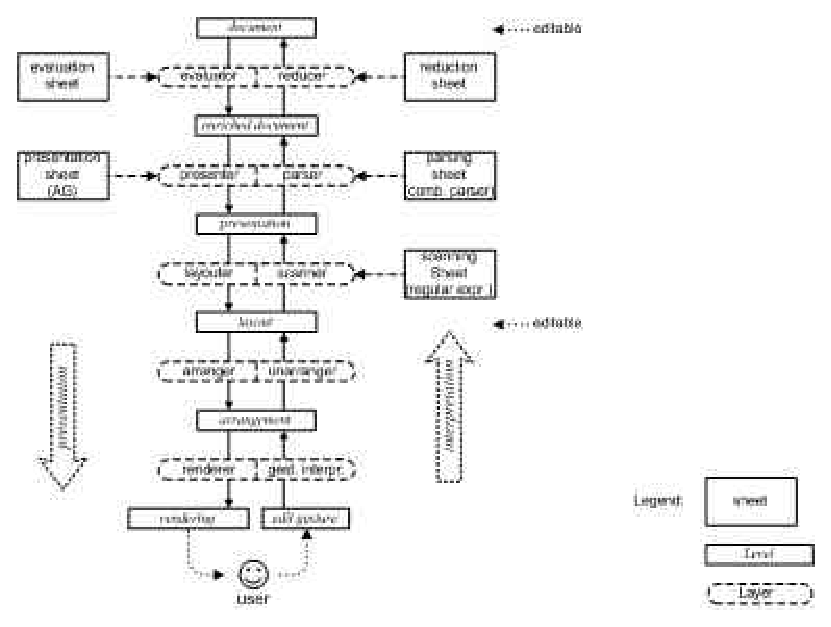
\includegraphics[width=12cm]{images/LayerOverview}
\caption{The levels and Layers of Proxima.}
\label{fig:levelsAndLayers}
\end{figure}

A data level in Proxima is not just an intermediate value in the presentation computation, but is an entity in its own right that maintains part of the state of the editor. The six data levels of Proxima are:


\bl
\o {\bf Document:} The document structure.

\o {\bf Enriched Document:} The document attributed with derived values and structures, such as the type of a function or a table of contents, typically computed by an attribute grammar~\cite{reps84synGen}.

\o{\bf Presentation:} A logical description of the presentation of the document, consisting of rows and columns of presentation elements with attributes. The presentation also supports formatting based on available space (e.g.\ line breaking).

\o{\bf Layout:} A presentation with explicit white space.

\o{\bf Arrangement:} A formatted layout with absolute size and position information.

\o{\bf Rendering:} A bitmap of the arrangement.
\el


\bc
We briefly discuss each of the five layers.

\head{Evaluation layer}\\
The evaluation layer takes care of computing derived structures and values over the document, and of mapping updates on these derived structures back to document updates. In this layer, for example, type inference may take place. The layer is parameterized by an {\em evaluation sheet} and a {\em reduction sheet}, which specify the mappings. 

\head{Presentation layer}\\
The presentation layer consists of the presenter and the parser. The presenter takes an enriched document tree and computes a presentation for it according to the {\em presentation sheet}. Its counterpart, the parser, maps a presentation tree back to an enriched document and is parameterized by a {\em parsing sheet}.

\head{Layout layer}\\
The layout layer handles automatic white space, which is maintained in the white-space map that is part of the presentation level. For each token, the layout component looks up the corresponding white space and inserts actual line breaks and spaces in the presentation. The scanner recognizes tokens in the layout level, based on regular expressions specified in the {\em scanning sheet}. It also stores white space in the white-space map. Because mapping tokens to strings is straightforward, the layout component does not need a sheet parameter.

\head{Arrangement layer}\\
In the presentation direction, the arrangement layer computes the precise position and size for each element in the layout level. It also handles line breaking. The arrangement level is not directly editable, so it need not be mapped back onto the layout level. Hence, the only thing that needs to be done in the interpretation direction, is to map absolute coordinates in edit commands to paths in the presentation tree. 

\head{Rendering layer}\\
The renderer creates a bitmap for the arrangement. In the other direction is the gesture interpreter, which maps edit gestures onto edit operations designated for the higher layers.

\ec

%\bl
%\o implementation: layer combinators.
%\o sometimes awkward, because we have to conform to the layers.
%\o but this has advantages: new GUI lib in a matter of days.
%\el




Presentation-oriented editing actually takes place at the layout level rather than the presentation level, thus allowing free-text editing also on white space (which is absent on the presentation level). Hence two levels that are directly editable: the document level, and the layout level. After an edit operation on the document, all levels from document to rendering are updated to reflect the update. After an edit operation on the layout level, the modified layout is scanned, parsed and reduced, to obtain the corresponding updated document, from which an updated rendering is computed. Scanning and parsing does not occur after every presentation edit operation. Depending on the editor, it may occur either on a navigation operation, after a certain time interval, or after an explicit request by the user.

In this paper, we will focus mainly on the presentation layer and layout layer, and, more specifically, on the scanner and parser in these layers. Because we do not refer to the evaluation layer, we will use the term document to refer to the enriched document. 
%Moreover, when it is clear from the context, we sometimes refer to the presentation of the document, when it is in fact the layout level rather than the presentation level.



%%%%%%%%%%%%%%%%%%%%%%%%%%%%%%%%%%%%%%%%%%%%%%%%%%%%
%
\section{The document structure}\label{sect:documentStructure}
%
%%%%%%%%%%%%%%%%%%%%%%%%%%%%%%%%%%%%%%%%%%%%%%%%%%%%

The document type in Proxima is a monomorphic (i.e.\ parameter free) Haskell data type with lists. Figure~\ref{fig:docType} shows the definition for a type \p{Decl} that represents declarations of simple expressions. This definition is the base from which a code generator creates a Haskell data type, as well as a number of utility functions.

\begin{figure}
\begin{center}
\begin{footnotesize}
\begin{verbatim}
data Decl = Decl ident:Identifier exp:Exp {idP1,idP2}

data Identifier = Ident str:String        {idP1}

data Exp = PlusExp  exp1:Exp exp2:Exp     {idP1}
         | DivExp   exp1:Exp exp2:Exp     {idP1}
         | PowerExp exp1:Exp exp2:Exp     {idP1}
         | IntExp   val:Int               {idP1}
\end{verbatim}
\end{footnotesize}
\end{center}
\caption{A document type for simple declarations.} \label{fig:docType} 
\end{figure}

The difference with Haskell syntax is that named fields are specified by putting an identifier and a colon in front of a child type. Furthermore, at the right of each constructor we have a number of identifiers that declare presentation identity fields, which refer to the tokens occurring in the presentation. For example, \p{Decl} has two fields, one for the equals sign and one for the semicolon, whereas \p{PlusExp} has only one, for the plus operator. A future version of Proxima will allow presentation identities to be specified in the presentation sheet rather than the document type. In the Haskell data type that is generated from this type definition, the presentation identity fields are placed in front of the other fields. Furthermore, two special constructors are added to each type by Proxima: a {\em hole} constructor for representing incomplete documents, and  {\em parse error} constructor for representing parse errors.

If we leave away the presentation identities, the declaration in Figure~\ref{fig:graphicalDecl} is represented by the value in Figure~\ref{fig:valueExample}. (The full version is provided in Section~\ref{sect:parseExample}.)

\begin{figure}
\begin{center}
\begin{footnotesize}
\begin{verbatim}
Decl (Identifier "x") 
     (PlusExp (DivExp (IntExp 1)
                      (PlusExp (PowerExp (IntExp 3) (IntExp 2))
                               (IntExp 5)))
              (IntExp 1))
\end{verbatim}
\end{footnotesize}
\end{center}
\caption{A value of type \p{Decl}.} \label{fig:valueExample} 
\end{figure}







%%%%%%%%%%%%%%%%%%%%%%%%%%%%%%%%%%%%%%%%%%%%%%%%%%%%
%
\section{The presentation process}\label{sect:presentationProcess}
%
%%%%%%%%%%%%%%%%%%%%%%%%%%%%%%%%%%%%%%%%%%%%%%%%%%%%

Before discussing the scanner and parser components, we briefly discuss their counterparts in the presentation direction: the presenter and layout components. The presenter component maps an (enriched) document onto the presentation level, according to rules in the presentation sheet, which is specified with an attribute grammar. The presentation itself is a value of type \p{Xprez}, computed in a compositional way, using the\ \p{Xprez} combinator language. After the presentation phase, the presentation level is mapped onto the layout level by the layout component. In the next three subsections, we introduce the language \Xprez, the attribute grammar formalism used in the presentation sheet, and the layout component.

\subsection{The {\Xprez} presentation language} \label{sect:xprez}

\Xprez\ is a combinator library for specifying graphical presentations with support for alignment and stretching.  The basic building blocks of \Xprez\ are text and graphical elements such as polygons, circles, and images. Combinators are used to combine presentations in rows and columns. The elements of a row or column are aligned along horizontal and vertical reference lines of their children, and do not overlap. Besides rows and columns, \Xprez\ also supports overlapping presentations and a flow layout for line breaking. We give an introduction to the language based on the example in Figure~\ref{fig:xprezFrac}. The function \p{frac} creates a graphical presentation of a fraction. 

The result of \p{frac (text "1") (text "1+x")} is~~\raisebox{-0.75ex}{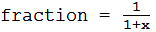
\includegraphics[width=0.5cm]{images/fracExample}}

\bc
Each presentation has a number of presentation attributes (e.g.\ color, font size, reference lines) that influence its appearance. Several functions are available for modifying presentation attributes. For example, for changing the font size, we can use \p{withFontsize :: Int -> Xprez -> Xprez}. \todo{mention \p{with}?}
\ec


\begin{figure}
\begin{center}
\begin{footnotesize}
\begin{verbatim}
frac :: Xprez -> Xprez -> Xprez
frac e1 e2 = let numerator   = hAlignCenter (pad (shrink e1) )
                 denominator = hAlignCenter (pad (shrink e2) )
             in  colR 2 [ numerator, vSpace 2, hLine
                        , vSpace 2, denominator ] `withHStretch` False
                        
pad xp = row [ hSpace 2, xp, hSpace 2 ]

shrink e = e `withFontSize_` (\fs -> (70 `percent` fs) `max` 10)
\end{verbatim}
\end{footnotesize}
\caption{The definition of \p{Frac}.} \label{fig:xprezFrac} 
\end{center}
\end{figure}

%\todo{one move for aligning hLine with + is not shown}

The \p{colR} combinator takes an argument that denotes which of its children provides the vertical reference line (in this case, the horizontal line in the fraction). The \p{withHStretch} function prevents the fraction from being horizontally stretchable. Finally, to shrink presentations, we use the combinator \p{withFontSize\_}, which takes a function argument that computes the new font size, given its previous value. Besides the combinators that produce presentations, \Xprez\ also has combinators for specifying edit operations in context menus, reactions to mouse clicks, and keeping track of document locations in the presentation.


\subsection{Document presentation}

For the presentation of the document, as well as for the computation of derived values and structures, Proxima uses the attribute grammar formalism. The presentation sheet is a file with an attribute grammar definition, which is compiled to a Haskell program by the Utrecht University AG compiler~\cite{swierstra08ag}.

For each type of node in the document, the presentation sheet defines a synthesized attribute \p{pres} of type \p{Xprez}. In the definition of \p{pres}, presentations of its children may be referred to. Besides the presentation, any number of attributes can be defined on the document tree. In this way we can easily add static checks or compute all variables in scope at some document location. Moreover, functions from external Haskell modules may be called, allowing for more complex computations, such as type checking.

% also possible edit operations specific to the doc node.

Each presentation rule states whether the presentation is parsing or structural. A parsing presentation consists of a sequence of tokens, which may be strings or structural presentations. In the presentation sheet, the top-most element of the parsing presentation (the one that is an immediate child of a structural presentation) must specify a parser, which is the parser to be applied to the sequence after it has been edited.

Since a structural presentation may not be edited at the presentation level, it is straightforward to map it back onto the document level, even if it has a graphical presentation. Hence, no parser needs to be specified in the presentation sheet.

%\todo{add structural example without id (slide?)}
Figure~\ref{fig:presentationSheet} shows three presentation rules for the declaration document type from Section~\ref{sect:documentStructure}. For brevity, the rules for \p{Ident}, \p{PowerExp}, and \p{IntExp} have been omitted. The Haskell type system enforces a parsing presentation to consist only of tokens and nested parsing presentations. Two functions are available for creating tokens: \p{token} and \p{structuralToken}. The first parameter of both functions is a presentation identity, which is one of the \p{idP} fields specified in the document type definition (Figure~\ref{fig:docType}). Note that we specify a parser for \p{Decl} because it is the top-level type, but also for \p{Exp}, since it may be a child of the structurally presented \p{DivExp} (or \p{PowerExp}). The definition of the parsers is provided in Section \ref{sect:parser}.

\begin{figure}
\begin{center}
\begin{footnotesize}
\begin{verbatim}
SEM Decl
  | Decl    loc.pres = parsing parseDecl [ @ident.pres, key @idP1 "="
                                         , @exp.pres, symb @idP2 ";" ]
SEM Exp
  | PlusExp loc.pres = parsing parseExp [ @exp1.pres
                                        , operator @idP1 "+"
                                        , @exp2.pres ]
  | DivExp  loc.pres = parsing parseExp [ structuralToken @idP1 $ 
                                          frac @exp1.pres @exp2.pres ]
                  
key      idp str = token idp str `withColor` blue
operator idp str = token idp str `withColor` green
sym      idp str = token idp str `withColor` orange
\end{verbatim}%$
\end{footnotesize}
\caption{Presentation sheet fragment.} \label{fig:presentationSheet} 
\end{center}
\end{figure}

% Maybe use this somewhere else
\bc  
To every presentation rule certain extra functionality is added implicitly, e.g.\ for managing the display of the focus and keeping track of document locations in the presentation tree. Such functionality could be supplied explicitly in the presentation sheet, but doing so is laborious and error prone. Hence, the presentation sheet contains definitions of local attributes \p{pres} rather than synthesized attributes. Automatically generated rules for the synthesized \p{pres} attributes add the default functionality to the local attribute.
\ec

\subsection{The layout component}

The main function of the layout component is to restore the implicit white space that is kept separately in the white-space map. Besides the white space, also the presentation focus is stored in the white-space map. This is necessary because parsing followed by presenting is not necessarily an identity mapping. After parsing, document structures represented by tokens may be presented graphically, and thus give rise to a restructured presentation. Recall that, typing a `\p{/}' in the Helium editor causes the introduction of a graphical fraction after parsing and presenting. The focus restoration mechanism takes care that after parsing and presenting the presentation focus remains at the same position. If the presentation focus cannot be restored from the tokens, the scanner will restore it by using its absolute coordinates in the presentation.

Apart from white space, the layout level has the same structure as the presentation level. Hence, we have {\em parsing} and {\em structural} layouts. The layout component is not parameterized by a sheet. The reason is that although we need a specification in order to create tokens from a string, the reverse process is straightforward, since each token contains its string representation.  





%%%%%%%%%%%%%%%%%%%%%%%%%%%%%%%%%%%%%%%%%%%%%%%%%%%%
%
\section{Scanning}\label{sect:scanner}
%
%%%%%%%%%%%%%%%%%%%%%%%%%%%%%%%%%%%%%%%%%%%%%%%%%%%%

The Proxima scanner maps character sequences in parsing layouts onto tokens, as specified in the scanning sheet. If the parsing layout contains any structural layouts, these are recursively scanned and recorded by special tokens.

\subsection{The \p{Token} type}

Tokens are represented by the type \p{Token}, of which a simplified version is shown in Figure~\ref{fig:tokenType}. A number of type parameters that are not important for this discussion are left out, as well as the constructors that have to do with Proxima's support for graph presentations. Each constructor has an \p{IDP} field that denotes its presentation identity number. Both \p{ParsingTk} and \p{StructuralTk} have a \p{Location} field that refers to the node in the document tree from the presentation of which the token originated. (Because \p{ErrorTk} tokens originate from the scanner they do not have this field.) The \p{Location} field is used when parsing structural layouts (which is explained in Section~\ref{subsect:parsingStructural}.) 


\begin{figure}
\begin{center}
\begin{footnotesize}
\begin{verbatim}
data Token Location userToken 
  = ParsingTk    IDP Location (Parser userToken) [Token node userToken]
  | StructuralTk IDP Location                    [Token node userToken]
  | UserTk       IDP userToken String 
  | ErrorTk      IDP String 
\end{verbatim}
\end{footnotesize}
\caption{The \p{Token} data type.} \label{fig:tokenType} 
\end{center}
\end{figure}

% Position is not shown ID has enough information
% Location

A {\bf\p{ParsingTk}} represents a parsing layout. The field \p{Parser userToken} is the parser that is used to parse the list of child tokens. This list contains no further \p{ParsingTk} tokens; tokens from all parsing descendents are collected and placed in the same list.

On the other hand, a {\bf \p{StructuralTk}} represents a structural layout and has a list of tokens for each of its child layouts. 

Finally, a {\bf \p{UserTk}} represents a string token, and an {\bf \p{ErrorTk}} is used to represent lexical errors. % Section~\ref{sect:parseScanErrors} explains its use.
%\todo{userTk also has Location, not shown here} \\
%\todo{Presentation arg has been removed, structurals are assumed not to have parse errors}


\subsection{Scanning the layout tree}

The scanner creates a tree of structural and parsing tokens that matches the structure of the layout level. Its behavior is determined by the kind of layout on which it is called.


% How the tokenizer works:
\head{Structural layout} A structural layout of a document node is an Xprez tree containing layouts stemming from the presentation of child nodes. The scanner traverses the layout tree and makes a recursive call on each child layout that is encountered. The list of child tokens is put in a \p{StructuralTk} and returned as the result of the scanner.

\head{Parsing layout} A parsing layout consists of a column of rows, which contain either strings or structural layouts. Each structural layout is mapped onto a structural token by recursively scanning it. The sequences of strings between the structural tokens are first extended with new-line characters to mark the transitions between rows. The resulting lists of characters are mapped onto lists of \p{UserTk} tokens according to the scanning sheet. The final list of child tokens is the result of merging the structural tokens with the recognized user tokens.


\subsection{The scanning sheet}

The lexical analysis of textual tokens is based on the Haskell lexical analyzer generator Alex~\cite{marlow07alex}, which is comparable to the lex and flex tools for C and C++. An editor designer has to define the data type \p{UserToken} and provide an Alex specification for the tokens. Figure~\ref{fig:scannerSheet} shows an example \p{UserToken} and scanning sheet. The Alex specification consists of a a number of macro definitions followed by a set of rules, each defining a token. A rule is a regular expression together with an action that constructs the token.

\begin{figure}
\begin{center}
\begin{footnotesize}
\begin{verbatim}
data 
  UserToken = 
    IdentToken String | OpToken String | SymToken Char | IntToken Int

$opChar = [\+ \- \=]
$symChar = [\;]
tokens :-
 $digit+                       { mkToken $ \s   -> IntToken (read s) }
 $opChar+                      { mkToken $ \s   -> OpToken s         }
 $symChar                      { mkToken $ \[c] -> SymToken c        }
 $lower [$alpha $digit \_ \']* { mkToken $ \s   -> IdentToken s      }
\end{verbatim}
\end{footnotesize}
\caption{Example \p{UserToken} and scanning sheet.} \label{fig:scannerSheet} 
\end{center}
\end{figure}
\bc
$lower = [a-z]
$upper = [A-Z]
$alpha = [$lower $upper]
$digit = 0-9		
\ec


\subsection{Handling white space}

In order to use the automatic white-space recognition, the following rule must be added to the scanning sheet:

\begin{footnotesize}
\begin{verbatim}
  [\n \ ]+        { collectWhitespace }
\end{verbatim} 
\end{footnotesize}

This rule causes the scanner to emit a special white-space token for each sequence of white space. A post-processing phase removes these white-space tokens, and records the trailing white space for each token in the white-space map. For the first token, also its leading white space is recorded. In case there are no tokens, any white space is associated with the presentation identity of the \p{ParsingTk} value that contains the list of tokens. 


The white-space model is currently somewhat limited, since white space is assumed to be a number of line breaks followed by a number of spaces. However, the model is easily extended to handle arbitrary white space and also comments that need to be treated similar to white space.






%%%%%%%%%%%%%%%%%%%%%%%%%%%%%%%%%%%%%%%%%%%%%%%%%%%%
%
\section{Parsing}\label{sect:parser}
%
%%%%%%%%%%%%%%%%%%%%%%%%%%%%%%%%%%%%%%%%%%%%%%%%%%%%

Unlike ordinary parsers, which take a list of tokens to produce a value, the Proxima parser is a function that takes only one token as input. This token can be either a structural token or a parsing token. In case of a structural token, the value is constructed automatically from the list of child tokens. If the token is a parsing token, its list of children is fed into the parser that was specified in the presentation sheet.

\subsection{Structural presentations}\label{subsect:parsingStructural}

A structural token corresponds to the presentation of a certain document node and contains a list of tokens that correspond to presentations of children of that document node. Each child may be presented multiple times, or even not at all. Furthermore, the order in which the child presentations appear may not correspond to the order of the children in the document node.

Nevertheless, we can parse a structural token automatically, since each child token contains a \p{Location} reference to the document node (and path) of which it is a presentation. Hence, for each token, we can determine the corresponding child of the document node. Because structural presentations are not editable at the presentation level, this information remains valid under presentation editing.

For child$_i$ of the document node, the parser takes the list of tokens corresponding to presentations of that child. If this list is empty, the presentation does not contain a presentation for the child, and we use its previous value, which is stored in the structural token. If the list is not empty, the token for the presentation that was edited is recursively parsed to yield a value for child$_i$. In case no presentation was edited, then the child value is also reused from the structural token for efficiency reasons. There will be at most one edited presentation, since Proxima does not allow editing multiple presentations of a single value at the same time. 

%\todo{check is not enforced yet}
%\todo{untyped, but safe}



\subsection{Parsing presentations}

The parser for a parsing presentation cannot be constructed automatically. Instead, we use the parser that was specified in the presentation sheet, which is stored in the \p{ParsingTk} value. Such parsers are specified using the UU Parsing library~\cite{swierstra03polishParsers, swierstra08parserCombinators}. This is a library for creating fast error correcting parsers with support for user-friendly error messages. Because of the error recovery, parsing does not stop after the first error, and hence multiple parse errors in different parts of the presentation can be reported. 
%\todo{The fact that they always produce a result is not used}

A Proxima parser is very similar to a regular parser specified with a combinator parser library. The only difference is that, in order to let the scanner handle white space and focus restoration, the presentation identities of the parsed tokens need to be stored in the appropriate fields of the document node. 

The list of tokens to which the parser is applied consists only of \p{UserTk}, \p{StructuralTk}, and \p{ErrorTk} tokens, since nested \p{ParsingTk} tokens are not created by the scanner. Primitive parsers are available for user tokens and structural tokens. No primitive parser is offered for error tokens, since these represent a lexical error by the scanner, which should always lead to a parse error.


Figure~\ref{fig:parser} shows the parsing sheet for the declaration type from the previous examples. The parser does not take into account priorities.
%\todo{mention that holes need to be explicitly parsed?}\todo{check code}

\begin{figure}
\begin{center}
%%%%%%%%%% max verbatim width, footnotesize %%%%%%%%%%%%%%%%%%%%%%%%%%%%
\begin{footnotesize}
\begin{verbatim}
parseDecl :: Parser Decl
parseDecl = (\id eqIdp exp semiIdp-> Decl eqIdp semiIdp id exp)
        <$> parseIdent <*> pToken (KeyToken "=") 
        <*> parseExp   <*> pToken (SymToken ';')
       
parseExp :: Parser Exp
parseExp = pStructural Node_Div
       <|> pStructural Node_Power
       <|> (\plusIdp e1 e2 -> PlusExp plusIdp e1 e2)
           <$> pToken (OpToken "+") <*> parseExp <*> parseExp
\end{verbatim}
\end{footnotesize}
\end{center}
\caption{Parsing sheet fragment for \p{Decl} and \p{Exp}.} \label{fig:parser} 
\end{figure}

The \p{pToken} parser is a primitive parser that succeeds on its argument \p{UserToken} value and returns the presentation identity of the token. The \p{pStructural} parser succeeds on a structural token for the constructor that is denoted by its argument. The argument has type \p{Node}, which is a generated type that represents the union of all constructors in the document type. 
%\todo{ add   \p{\\UserTk (IntToken i) -> <\$> pTokenEx (IntToken 0)}?? }%$

Note that we do not restore the presentation identity of the \p{ParsingTk} value itself in the \p{Exp} parser. The reason is that this is only necessary if the parser accepts an empty list of tokens. This is not true for the expression parser, so when only white space is present, a parse error is returned, which takes care of handling the white space. For a top-level parser that does accept an empty token list (e.g.\ a parser for a list of declarations), a special combinator is available that provides the parser with the presentation identity of the \p{ParsingTk} value.

Although Proxima currently uses the UU Parsing library, this connection is not fixed. In fact, any  parser library that is parameterized with its input token type is suitable. Hence, a binding with for example the Parsec library~\cite{leijen08parsec} is also possible. The only thing that needs to be done in order to use a different library is to define a primitive parser \p{pStructural} and a combinator that applies a parser and returns an error value in case of a parse error.

\subsection{Example} \label{sect:parseExample}

As an example for the parser, we show the result of parsing the tokens in Figure~\ref{fig:scanResult} that were obtained from scanning ~\raisebox{-1.43ex}{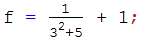
\includegraphics[width=1in]{images/scanFrac}} 

Figure~\ref{fig:parseResult} contains the resulting document structure. The value is in fact the example from Section~\ref{sect:documentStructure} with the presentation identities shown as subscripts. The presentation identities correspond to the identities of the tokens in Figure~\ref{fig:scanResult}. The \p{Decl} node has two presentation identities: $2$ for the equals sign and $16$ for the semicolon. All other nodes have only one. 

\begin{figure}
\begin{center}
\begin{footnotesize}
\begin{tabbedCode}
Decl$_{2,16}$ \= (Identifier$_1$ "x")\\ 
              \> (PlusExp$_{14}$ \= (DivExp$_3$ \= (IntExp$_5$ 1) \\
              \>                 \>             \> (PlusExp$_{12}$ \= (PowerExp$_7$ (IntExp$_9$ 3) (IntExp$_{11}$ 2))\\
              \>                 \>             \>                 \> (IntExp$_{13}$ 5)))\\
              \>                 \>(IntExp$_{15}$ 1))
\end{tabbedCode}
\end{footnotesize}
\end{center}
\caption{A parsed declaration.} \label{fig:parseResult} 
\end{figure}

\subsection{Parse errors} \label{sect:parseScanErrors}

On a parse error, a parser does not return a document tree, which means there will not be a document to present. To account for this, the parser returns the special value for which a constructor was added to each type in the document. For a document type $Type$, this constructor reads:

\begin{footnotesize}
\begin{tabbedCode}
data $Type$ \= =\\
            \> ...\\
            \> | ParseErr\_$Type$ IDP [ErrorMessage] [Token node userToken] 
\end{tabbedCode}
\end{footnotesize}

When a parse error is encountered, the parser constructs a \p{ParseErr} value and supplies it with a list of error messages and the list of tokens it tried to parse. The presentation identity comes from the parsed \p{ParsingTk} value and is used to handle white space in absence of tokens. The presenter uses the list of tokens when the parse error node is to be presented. In addition, squiggly lines are placed at the presentation of each token that is referred to by the error-message list. The white space for the tokens in the parse error node was already handled by scanner, and is restored by the layout component in the same way as it is for tokens stemming from ordinary presentations.

Each type of node in the document has a (generated) synthesized attribute \p{parseErrors}, which is the collection of all parse errors in the nonterminal or its descendents. This attribute can be used to show a list of parse errors in the presentation. 


% lexical errors
Lexical errors require a special treatment. When Alex encounters a lexical error, it stops at the offending character. The offending character and the remainder of the input are put in an \p{ErrorTk} token, which will always cause a parse error since no primitive parser is offered that accepts it. Since scanning the string stops at the offending character, all following white space  will be recorded in the string, rather than stored in the white-space map. Therefore, the layout component treats error tokens specially by expanding any white space encoded in the string. %\todo{interpretation extra state in parsing will require storing ScanChars rather than chars}






%%%%%%%%%%%%%%%%%%%%%%%%%%%%%%%%%%%%%%%%%%%%%%%%%%%%
%
\section{Related work}\label{sect:relatedWork}
%
%%%%%%%%%%%%%%%%%%%%%%%%%%%%%%%%%%%%%%%%%%%%%%%%%%%%

Most structure editors can be categorized as either syntax-directed (deriving a presentation from the document structure) or syntax-recognizing (deriving the structure from the presentation). Syntax directed editors, such as the Synthesizer Generator~\cite{reps84synGen}, LRC~\cite{saraiva00lrc}, SbyS~\cite{magnusson90orm}, and Redwood~\cite{westphal04redwood} allow graphical presentations, but do not provide a parser for editing mixed presentations. On the other hand, syntax recognizing editors, such as Pan~\cite{ballance92pan} and Harmonia~\cite{boshernitsan01harmonia} support presentation-oriented editing, but do not allow mixed graphical presentations.

Examples of systems that do support editing (and parsing) of mixed presentations are editors for mathematical formulas, such as Amaya~\cite{amaya08}, MathSPad~\cite{verhoeven00mathspad} and the commercial system Mathematica. However, these systems work for a fixed document type, and are not easily extensible. Somewhat more general, Eisenberg and Kiczales describe a presentation extension formalism~\cite{eisenberg07presExtension} for Eclipse, but their solution is targeted at extending Java only.

The Barista framework~\cite{KoMyers06Barista} has similarities to Proxima, although it is targeted mainly at code editors. The system allows graphical presentations for program structures, but these are expanded to the underlying textual presentation when edited. Although this is good to have as optional behavior, it is in many cases unnecessary.

\bc
older systems either had text only synthesizer generator, asfsdf. Or purely structural visual redwood + some other visual langs, but then no free text editing.


More modern is Barista. Allows graphical views. However, when editing the view, it is expanded to its sequential representation. Good as an option, but in many cases unnecessary. 



\noindent Barista~\cite{KoMyers06Barista} is a powerful framework for building code editors. It is built on top of Citrus~\cite{KoMyers05Citrus}, which is a UI toolkit together with an object-oriented language. Although Barista is targeted at code editors, the presentation of the code can be visual, for example allowing for images to appear in comments, or having graphical presentations of code. The editors created with Barista are syntax directed, but presentation-oriented editing is available. 

\ec



%%%%%%%%%%%%%%%%%%%%%%%%%%%%%%%%%%%%%%%%%%%%%%%%%%%%
%
\section{Conclusion}\label{sect:conclusion}
%
%%%%%%%%%%%%%%%%%%%%%%%%%%%%%%%%%%%%%%%%%%%%%%%%%%%%


Editors for programming languages can benefit much from editable graphical presentations of programs. Such graphical presentations, however, cannot be parsed with conventional parsing techniques. In this paper, we introduced a method for scanning and parsing mixed textual and graphical presentations. A combinator parser is used for textual parts of the presentations, whereas the graphical parts are recognized automatically, based on information in the presentation itself. The scanner and parser are part of the Proxima generic editor, and have been used to implement a number of prototype editors.
\bc
The Proxima system is still under development. No special attention to incrementality. Current parsers are fast. In a background thread. Scanner also not incremental, although quite easy to realize. Tests will have to show if this is nec.

The parsing method described in this paper allows for easy construction Allows editors to finally let go of ascii and provide a rich view ...
\ec
\bc
\bl
\o document extra state in parsing presentations not shown here.
\el

\bl
\o comments can be handled similar to white space and focus
\o more static checks are possible
\o easy ways to increase speed after change management
\o Proxima allows building IDE with only little effort.
\o use ag to add static/type checks
\el
\ec


%%%%%%%%%%%%%%%%%%%%%%%%%%%%%%%%%%%%%%%%%%%%%%%%%%%%
%
% References

\bibliographystyle{sbc}
\bibliography{../proxima}

\end{document}
